\section{introduction}

\textbf{Faser i traditionel softwareudvikling}
\begin{enumerate}
	\item{Foranalyse}
	\item{Analyse}
	\item{Design}
	\item{Implementering/programmering}
	\item{Test}
	\item{Idriftsættelse/deployment}
	\item{Drift/vedligeholdelse}
	\item{Udfasning}

\end{enumerate}

\textbf{Typer as systemer}

\begin{itemize}
	\item{Informationssystemer (IS) er forholdsvis store applikationer som håndterer store datamængder
	            og interagerer med andre systemer.}
	\item{Indlejrede systemer som regel forholdsvis små og har en vandtæt specifikation.}
	\item{Kunstig intelligens og/eller maskinlæring, går kort fortalt ud på at
	            løse vanskelige problemer}
\end{itemize}


\textbf{Database Management Systems (DBMS)}

Et databasesystem skal muliggøre oprettelse af databaser ved at definere deres struktur med et
data definition language. Det skal også tillade brugere at udføre forespørgsler og ændre data
ved hjælp af et data manipulationsprog. Systemet skal understøtte langvarig lagring af store datamængder, sikre
datakonsistens selv ved nedbrud, og håndtere samtidige brugeradgange på en måde, så deres handlinger
ikke fører til inkonsistente data.

\textbf{Relationelle database systemer}

Tom Codd fremsatte sin relationelle model i 1970. Her skulle data organiseres i tabeller, kaldet relations.
Brugeren skulle ikke bekymre sig om den faktiske lagring af data - det håndteres behind the scenes.
Tilgang til databasen fandt sted ved hjælp af et højniveau sprog kaldet \emph{structured query language}(SQL).

\textbf{Entity relationship diagram - ERD}

Beskriver relationen mellem de forskellige tabeller. I et ER-diagram modelleres en 1:M relation
(fx en fiskeart kan indgå i mange fangster), således at foregreningen af den ene ende af forbindelsen
mellem tabellerne vender ind imod den tabel, hvor fremmednøglen er.

\begin{center}[H]
	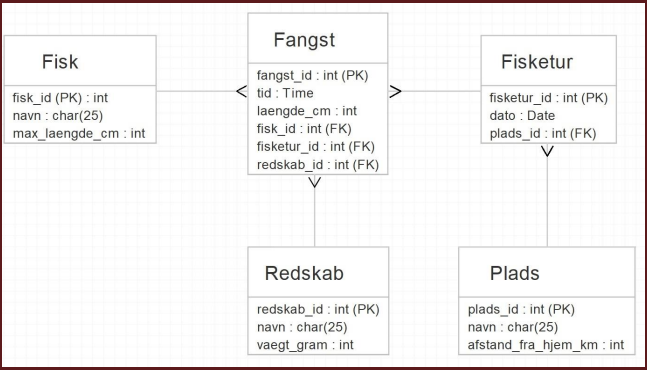
\includegraphics[width=0.6\textwidth]{Images/ERD.png}
\end{center}
